%!TEX TS-program = pdflatex
%!TEX encoding = UTF-8 Unicode
%!TeX spellcheck = it_IT

\documentclass{book}
\usepackage{graphicx}
\usepackage[italian]{babel}	% language
\usepackage[utf8x]{inputenc} % codec
\usepackage{amsmath}	% formulas
\usepackage[pdftex,
            pdfauthor={Marco Romanelli},
            pdftitle={TITOLOTESI},
            pdfsubject={SOGGETTOTESI},
            pdfkeywords={PAROLECHIAVETESI}]{hyperref}	% hyperlinks
\usepackage{algorithm}	% pseudocode for algorithms
\usepackage[noend]{algpseudocode} % same as above
\usepackage{mymacros} % macros
\usepackage{xcolor} % for colors (like in codes)
\usepackage{colortbl} %
\usepackage{listings}	% code
\definecolor{codegreen}{rgb}{0,0.6,0}
\definecolor{codegray}{rgb}{0.5,0.5,0.5}
\definecolor{backcolor}{rgb}{0.98,0.98,0.98}
\definecolor{RoyalBlue}{rgb}{0.25, 0.41, 0.88}
\definecolor{Peach}{rgb}{1.0, 0.9, 0.71}
\definecolor{SeaGreen}{rgb}{0.18, 0.55, 0.34}
\definecolor{gray}{rgb}{0.4,0.4,0.4}
\definecolor{darkblue}{rgb}{0.0,0.0,0.6}
\definecolor{cyan}{rgb}{0.0,0.6,0.6}

\renewcommand{\lstlistingname}{Codice}% Listing -> codice
\renewcommand{\lstlistlistingname}{Frammenti di codice}% List of Listings -> Frammenti di codice

\lstdefinestyle{mystyle}{
    backgroundcolor=\color{backcolor},
    commentstyle=\color{Peach}\ttfamily,
    keywordstyle=\color{RoyalBlue},
    numberstyle=\tiny\color{codegray},
    stringstyle=\color{SeaGreen}\ttfamily,
    basicstyle=\footnotesize\ttfamily,
    breakatwhitespace=false,
    breaklines=true,
    captionpos=b,
    keepspaces=true,
    numbers=left,
    numbersep=5pt,
    showspaces=false,
    showstringspaces=false,
    showtabs=false,
    tabsize=2,
    frame=trbl, % draw a frame at the top, right, left and bottom of the listing
	frameround=ftff, % angolo in basso a destro curvo
	framesep=4pt, % quarter circle size of the round corners,
	inputencoding=utf8x,
    %extendedchars=true,
    %literate={á}{{\'a}}1 {à}{{\`a}}1 {é}{{\'e}}1 {è}{{\`e}}1 {ù}{{\`u}}1 {ò}{{\`o}}1 {ì}{{\`i}}1,
    belowskip=1em,
    aboveskip=1em,
}
\lstset{style=mystyle}

\lstdefinelanguage{JavaScript}
{
  % list of keywords
  morekeywords={ true, false, catch, function, break,	new, class, extends, var, require, switch, return, import, if, while, for, this, View, Text, StyleSheet},
  sensitive=false, % keywords are not case-sensitive
  morecomment=[l]{//}, % l is for line comment
  morecomment=[s]{/*}{*/}, % s is for start and end delimiter
  morestring=[b]' % defines that strings are enclosed in double quotes
}

\lstdefinelanguage{Properties}
{
	% list of keywords
	morekeywords={ true, false, catch, function, break,	new, class, extends, var, require, switch, return, import, if, while, for, this, View, Text, StyleSheet},
	sensitive=false, % keywords are not case-sensitive
	morecomment=[l]{\#}, % l is for line comment
	morecomment=[s]{/*}{*/}, % s is for start and end delimiter
	morestring=[b]' % defines that strings are enclosed in double quotes
}

\lstdefinelanguage{JSON}
{
  % list of keywords
  morekeywords={string, boolean, int, Array, Node, Asset, AssetDetail, Filter, FilterItem},
  sensitive=false, % keywords are not case-sensitive
  morecomment=[l]{//}, % l is for line comment
  morecomment=[s]{/*}{*/}, % s is for start and end delimiter
  morestring=[b] % defines that strings are enclosed in double quotes
}

\colorlet{punct}{red!60!black}
\definecolor{background}{HTML}{EEEEEE}
\definecolor{delim}{RGB}{20,105,176}
\colorlet{numb}{magenta!60!black}

\lstdefinelanguage{json}{
    basicstyle=\normalfont\ttfamily,
    numbers=left,
    numberstyle=\scriptsize,
    stepnumber=1,
    numbersep=8pt,
    showstringspaces=false,
    breaklines=true,
    frame=lines,
    backgroundcolor=\color{background},
    literate=
     *{0}{{{\color{numb}0}}}{1}
      {1}{{{\color{numb}1}}}{1}
      {2}{{{\color{numb}2}}}{1}
      {3}{{{\color{numb}3}}}{1}
      {4}{{{\color{numb}4}}}{1}
      {5}{{{\color{numb}5}}}{1}
      {6}{{{\color{numb}6}}}{1}
      {7}{{{\color{numb}7}}}{1}
      {8}{{{\color{numb}8}}}{1}
      {9}{{{\color{numb}9}}}{1}
      {:}{{{\color{punct}{:}}}}{1}
      {,}{{{\color{punct}{,}}}}{1}
      {\{}{{{\color{delim}{\{}}}}{1}
      {\}}{{{\color{delim}{\}}}}}{1}
      {[}{{{\color{delim}{[}}}}{1}
      {]}{{{\color{delim}{]}}}}{1},
}

\lstdefinelanguage{URM}
{
	% list of keywords
	morekeywords={ S, J, T, Z, I},
	sensitive=false, % keywords are not case-sensitive
	morecomment=[l]{//}, % l is for line comment
	morecomment=[s]{/*}{*/}, % s is for start and end delimiter
	morestring=[b]' % defines that strings are enclosed in double quotes
}

\lstdefinelanguage{RDFA}{
	language=html,
	sensitive=true,
	alsoletter={<>=-},
	ndkeywords={
		% General
		=,
		% HTML attributes
		charset=, id=, width=, height=, property=, about=, rel=, rev=, prefix=, vocab=, content=, datatype=
	},
	morecomment=[s]{<!--}{-->},
	tag=[s]
}

\lstdefinestyle{BashStyle}{
  language=bash,
  basicstyle=\small\sffamily,
  numbers=left,
  numberstyle=\tiny,
  numbersep=3pt,
  frame=tb,
  columns=fullflexible,
  backgroundcolor=\color{yellow!20},
  linewidth=0.9\linewidth,
  xleftmargin=0.1\linewidth,
  framexleftmargin=0.2em}

\lstdefinestyle{myJSON}{
    language=json,
    basicstyle=\tiny,
	numbers=none}


% \lstdefinestyle{makefile}{
%   otherkeywords={.SUFFIXES},
%   alsoletter={:},
%   morekeywords=[1]{SUFFIX, CPP_},
%   morekeywords=[2]{vasp:,makeparam:,zgemmtest:,dgemmtest:,ffttest:,kpoints:,clean:},
%   style=global,%
%   morecomment=[l][commentstyle]{\#},%
%   emphstyle={\color{vimvert}},%
%   moredelim=[s][\color{vimvert}]{\$(}{)}%
%   }

\lstdefinelanguage{XML}
{
  morestring=[b]",
  morestring=[s]{>}{<},
  morecomment=[s]{<?}{?>},
  stringstyle=\color{black},
  identifierstyle=\color{darkblue},
  keywordstyle=\color{cyan},
  morekeywords={xmlns,version,type}% list your attributes here
}
 %
\lccode`~=0 %

\graphicspath{{figures/}}	% image path

\begin{document}

%!TEX TS-program = pdflatex
%!TEX encoding = UTF-8 Unicode
%!TeX spellcheck = it_IT
%!TEX root = ../tesi.tex
%
\chapter{Contesto e lavori correlati}
%
\section{Introduzione}
% TODO in progess...
%% PASSI:
% - introdurre le vanet
% - importanza della propagazione/protocolli broadcast
% - importanza delle simulazioni
% - importanza di simulazioni veritiere
% - (~) modelli per rendere migliori le simulazioni
% - importanza degli ostacoli
% - modellazione di ambiente 3d
% - struttura documenti tesi
%
I recenti progressi tecnologici nell'hardware, software e nell'ambito delle telecomunicazioni hanno permesso
l'ideazione e lo sviluppo di diverse tipologie di reti, impiegate poi in un'ampia gamma di scenari.
%
% % I recenti progressi tecnologici nell'hardware, software e nell'ambito delle telecomunicazioni hanno permesso
% % l'ideazione e lo studio di vari tipologie di reti, impiegate poi in un'ampia gamma di scenari.
% Le reti veicolari (\textit{Vehicular Ad-hoc Networks}, VANET) stanno, negli ultimi anni, riscuotendo un crescente interesse
% grazie ai recenti progressi tecnologici e ai molteplici casi di studio, dalla sicurezza dei veicoli e delle strade e allo sviluppo di applicazioni
% multimediali intra-veicolari.
% % Vista l'impossibilità per un'infrastruttura centrale di garantire una copertura totale, un settore della ricerca % mah
% % verte sullo studio di protocolli di comunicazione intelligenti in grado di propagare informazioni velocemente.
% % Per la progettazione e la verifica di questi spesso si utilizzano simulazioni software in grado di analizzare
% % diversi scenari limitando i costi di sviluppo.
%

% struttura documento tesi
% TODO: inserire referenze ai capitoli
Il lavoro è strutturato come segue.
Nel capitolo seguente verrà presentato il protocollo Fast Broadcast, la fase di stima e quella di inoltro per finire poi con l'estensione in due dimensioni.
Il Capitolo 3 analizzerà il modello a ostacoli, sia dal punto di vista matematico che da quello analitico inerente alla simulazione;
concluderà presentanto l'estenzione tridimensionale.
Il Capitolo 4 darà una veloce panoramica sui software utilizzati, fra cui ns-3 e SUMO.
Il Capitolo 5 illusterà le tipologie di simulazioni effettuate e i relativi risultati ottenuti.
Seguiranno le conclusioni nel Capitolo 6, evidenziando alcuni possibili sviluppi.
% In appendice è possibile trovare
%
\section{Modelli di radiopropagazione}
Un modello di radiopropagazione (MRP) simula gli effetti dell'attenuazione del segnale radio (segnali elettromagnetici nello spazio libero o etere, in contrasto con la propagazione guidata)
dovuta alla distanza, cammini multipli per effetto della riflessione, ombreggiatura causata da grandi ostacoli come edifici.
L'utilizzo di un'idonea rappresentazione per questo tipo di ostacoli è, quindi, necessaria nel contesto di simulazioni di reti VANET (\textit{Vehicular Ad-hoc Networks}) in ambienti urbani
e suburbani.

Nel corso degli anni, diversi MRP sono stati proposti.
Il più semplice di questi si chiama modello a disco unitario (\textit{unit-disk model}), nel quale i veicoli possono comunicare fra loro se si trovano entro una certa soglia
di distanza, mentre non possono altrimenti~\cite{6554832}.
Un modello molto utilizzato nelle simuazioni di VANET è il modello a doppio raggio (\textit{Two-ray ground-reflection model}),
nel quale il segnale in fase di ricezione è composto da una componente in linea diretta e una seconda derivante dalla riflessione causata dal terreno~\cite{DBLP:books/daglib/0091821}.
In~\cite{Schmitz:2006:ERW:1164717.1164730} e in~\cite{Souley2005RealisticUS}, modelli più sviluppati prendono in considerazione anche le properità riflettenti delle superfici e degli ostacoli.

Tuttavia, un approcio diretto di questo tipo difficilmente scala al numero di nodi necessario in un classico scenario VANET e per questo motivo
spesso questi modelli si affidano a una fase di pre-elaborazione che può richiedere tempi elevati~\cite{Stepanov:2008:IMR:1293378.1293656}.
Per ovviare a questo problema, alcune proposte astraggono dalle informazioni sui singoli edifici, modellando l'ambiente urbano in modo omogeneo
così da creare un modello analitico per l'ombreggiatura~\cite{1492678}.
Questo tipo di modelli riducono il costo computazionale e generalmente si raffrontano bene con i risultati reali;
ciò nonostante, non riescono a catturare effetti a livello mesoscopico, come eventuali spazi fra edifici che permetterebbero trasmissioni a corto raggio~\cite{Giordano:2010:CST:1860058.1860065}.

Sono affetti dallo stesso problema anche i modelli (puramente) probabilistici, in quanto non tengono in considerazione la geometria urbana sottostante.
Questi modellano l'effetto dell'ombraggiatura tramite distribuzione stocastiche, fra cui Rice, Rayleigh, Nakagami-m, lognormale e Weibull~\cite{6554832}~\cite{Rappaport:2001:WCP:559977},
%
\section{Modellazione di ostacoli}
Nelle simulazioni di alcuni scenari, come possono essere le VANET, un'accurata rappresentazione della topologia dell'ambiente è necessaria,
in quanto questa limita non solo la mobilità dei veicoli ma interferisce anche con le trasmissioni radio~\cite{7543980}~\cite{amjad2015impact}.
L'attenuazione radio viene spesso modellata in modo deterministico basandosi principalmente sulla distanza della visuale (\textit{Line Of Sight}, LOS)
fra i veicoli, aggiungendo i modelli stocastici per considerare l'ombreggiatura.

Negli ultimi anni, diversi studi hanno cercato di rappresentare l'effetto ombreggiatura causato dagli edifici.
In~\cite{Giordano:2010:CST:1860058.1860065}, gli autori utilizzavano tecniche di geocodifica inversa (\textit{reverse geocoding}) per estrapolare
informazioni sulla topologia della rete stradale in stile Manhattan. Da qui, veniva derivata la geometria degli edifici utilizzata
per differenziare i casi in cui i due veicoli comunicanti avessero la visuale libera (LOS) o meno (\textit{Non Line Of Sight}, NLOS)
e calcolare di conseguenza la potenza del segnale in ricezione.
In~\cite{4020783}, invece, le informazioni sugli edifici erano codificate direttamente all'interno dell'ambiente sviluppato, chiamato
EGRESS (\textit{Enviroment for Generating REalistic Scenarios for Simulations}), e permettavano di definire tre tipologie di edificie altrettanti
percorsi per simulare la mobilità dei nodi; il modello permette anche di configurare, con alcuni limiti, diversi tipi di materiale dei pavimenti e dei muri degli edifici.
Gli autori di~\cite{Carpenter:2015:OMI:2756509.2756512} prendevano le informazioni per la geometria degli edifici da una piattaforma gratuita
chiamata OpenStreetMap (OSM)~\cite{osmWebsite}; poi queste venivano elaborate da un software per la simuazione della mobilità di veicoli
che generava un file contenente i dati sugli edifici e un altro per la mobilità dei veicoli;
il modello di propagazione teneva conto della distanza interna percorsa del segnale e del numero di muri esterni che questo attraversava.
% NB: ultima parte non bellissima

%!TEX TS-program = pdflatex
%!TEX encoding = UTF-8 Unicode
%!TeX spellcheck = it_IT
%!TEX root = ../tesi.tex

\chapter{Protocollo FB}
La tecnica del Fast Broadcast \cite{Palazzi07howdo} si compone di due fasi. La prima, chiamata ``Fase di stima'', permette a ogni veicolo di avere una stima aggiornata
del proprio raggio trasmissivo. La seconda, invece, è detta ``Fase di inoltro'' viene attivata nel momeno in cui si renda necessario inviare un messaggio
a tutti gli altri veicoli nell'area di interesse.

\section{Fase di stima}

%!TEX TS-program = pdflatex
%!TEX encoding = UTF-8 Unicode
%!TeX spellcheck = it_IT
%!TEX root = ../tesi.tex
%
\chapter{\textit{Obstacle Shadowing Model}}
\section{ns-3}
I Network Simulator (ns)~\cite{ns3Website} sono una serie di simulatori a eventi discreti utilizzati principalmente in ambito accademico e di ricerca.
La terza versione, ns-3, creta nel 2006 da Tom Henderson, George Riley, Sally Floyd e Sumit Roy, è stata riscritta da zero utilizzando \Cpp e abbandonando
la retrocompatibilità con ns-2; il software è distribuito sotto licenza GNU GPLv2.
%
\section{Il modello matematico}
Gli autori di~\cite{Carpenter:2015:OMI:2756509.2756512} riprendono il modello introdotto da Christoph Sommer et al.\ in~\cite{5720204},
nel quale la perdita di segnale dovuta a ostacoli $L_{s,o}$ dipende dall'attenuazione causata dai bordi dell'ostacolo (\textit{per-wall attenuation})
e quella derivante dalla superficie interna (\textit{per-meter attenuation}):
\begin{gather}\label{eq:osbtacle-model}
	L_{s,o} = \alpha n + \beta d_o
\end{gather}
Nella formula precedente, $n$ indica il numero di volte che il bordo dell'ostacolo viene intersecato dalla visuale (of LoS, da \textit{Line of sight}),
mentre $d_o$ è la distanza, in metri, attraversa all'interno dell'ostacolo.
Il parametro $\alpha$ rappresenta l'attenuazione per-metro espressa in decibels (dBm), invece
$\beta$ l'attenuazione per-metro, sempre in decibels (dB/m).

I due fattori di calibrazione permettono di rappresentare più tipologie di edificio.
I valori predefiniti di $\alpha = 9$ dBm e $\beta = 0,4$ dB/m sono buoni per la maggior parte delle applicazioni
anche se, naturalmente, non per tutte.
Riportando l'esempio in~\cite{5720204} di una casa in costruzione, il modello riesce a rappresentare le caratteristiche dell'attenuazione,
tuttavia i parametri sono distanti da quelli sopra indicati: $\alpha$ = 2.4 dBm and $\beta$ = 0.63 dB/m.
%
\begin{figure}[!h]
	\centering
	\begin{center}
		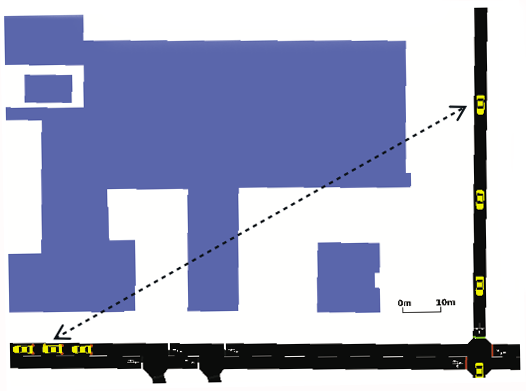
\includegraphics[width=.8\textwidth]{carpenter-1.png}
	\end{center}
	\label{fig:scenario-urbano-1}\caption{Esempio di scenario urbano.}
\end{figure}
%
Prendiamo l'esempio raffigurato in Figura~\ref{fig:scenario-urbano-1}, dove la linea fra i due veicoli interseca $n=6$ muri e una distanza interna di $d_o=32$m;
sostituendo i valori in~\ref{eq:osbtacle-model} si ottiene: $L_{s,o} = 9*6 + 0,4*32 = 66,8$dB.
Si evince come, con questa quantità di attenuazione, sia difficile che la trasmissione da un veicolo abbia abbastanza potenza per essere ricevuta dal secondo veicolo.
%
\section{L'implementazione}
Nel dettaglio, gli ostacoli sono rappresentati da poligoni bidimensionali che ne definiscono i bordi (spigoli).
Riprendendo l'esempio in Figura~\ref{fig:scenario-urbano-1}, la linea di visibilità (in questo caso \textit{obstructed-line-of-sight}, OLOS), fra i due veicoli potrebbe
intersecare diversi muri e percorrere una certa distanza internamente a uno o più edifici.
Il modello \textit{Obstacle Shadowing} conta il numero di intersezioni con gli spigoli dell'ostacolo, calcola la distanza percorsa internamente a esso e, utilizzando
il modello matematico visto in precedenza, restituisce l'attenuazione della trasmissione wireless fra i due veicoli.

Il tutto è implementato in ns-3 tramite tre classi: \textsf{Obstacle} contiente la rappresentazione geometrica dell'ostacolo, utilizzando le Computational Geometry Algorithms Library (CGAL),
come anche i parametri dell'attenuazione per-metro e per-muro.
\textsf{Topology} legge i dati degli edifici da un file specifico, generato dall'utility Polyconvert del software SUMO (Simulator for Urban Mobility)~\cite{sumoWebsite}
a partire dalle informazioni ottenute da OpenStreetMap (OSM)~\cite{osmWebsite}.
L'oggetto \textsf{Topology} così creato è poi utilizzato per determinare la perdita di segnale fra due punti (e.g. veicoli), utilizzando l'algoritmo illustrato
in Figura~\ref{fig:algoritmo-getobstucteddistancebetween}.
%
\begin{algorithm}[!h]
\caption{Algoritmo per determinare il numero di intersezioni con i bordi dell'ostacolo e la distanza interna percorsa fra due punti.}\label{fig:algoritmo-getobstucteddistancebetween}
\begin{algorithmic}[1]
	\Procedure{GetObstuctedDistanceBetween}{$p_1, p_2, B$}
	\BState{}\emph{Input}: $p_1, p_2$: posizione dei due veicoli; $B$: partizione binaria dello spazio (BSP) di ostacoli.
	\BState{}\emph{Output}: Distanza interna percorsa, $m_o$, e il numero di intersezioni con i bordi, $n$.
	\State{$m_o \gets 0;\; n \gets 0$}
	\TextState{Inizliazza la portata massima $r$: distanza dal punto $p_1$ o $p_2$ al centro di un ostacolo, utilizzata per filtrare il sottoinsieme di ostacoli sufficientemente vicini.}
	\TextState{Crea un riquadro di delimitazione $b$ per $p_1$ e $p_2$ ed estendila di $r$ in tutte le direzioni.}
	\TextState{Calcola l'insieme di potenziali ostacoli $O$ da quelli all'interno di $b$ in $B$.}
	\ForEach{ostacolo $o \in O$}
		\If{(distance($p_1$, o.center) $< r$) OR (distance($p_2$, o.center) $< r$)}
			\ForEach{spigollo $e \in o$}
				\If{$s$ interseca un raggio da $p_1$ a $p_2$}
					\State{$n \gets n+1$}
					\TextState{Salva la distanza minima e massima da $\{ p_1, p_2\}$ al punto d'intersezione.}
				\EndIf{}
				\TextState{$m_o \gets m_o+$ differenza fra i valori min e max calcolati al passo precedente.}
			\EndFor{}
		\EndIf{}
	\EndFor{}
	\Return{$m_o$ e $n$}
	\EndProcedure{}
\end{algorithmic}
\end{algorithm}
%

%!TEX TS-program = pdflatex
%!TEX encoding = UTF-8 Unicode
%!TeX spellcheck = it_IT
%!TEX root = ../tesi.tex
%
\chapter{Software}
%
\section{Network Simulator 3}
Network Simulator 3 (ns-3)~\cite{ns3Website} è un simulatore a eventi discreti utilizzato principalmente in ambito accademico e di ricerca,
scritto in \Cpp e Python; è un software libero distribuito sotto licenza GNU GPLv2.
Creato nel 2006 da un gruppo coordinato da Tom Henderson, George Riley, Sally Floyd e Sumit Roy con lo scopo
di ovviare ad alcune grosse limitazioni della precedente versione (ns-2), come ad esempio la necessità di utilizzare
un linguaggio di \textit{scripting} dedicato per modellare le simulazioni o una maggiore scalabilità~\cite{Henderson:2006:NPG:1190455.1190468}.
Attualmente è l'unica versione della serie a essere sviluppata.
È d'obbligo menzionare che, sebbene tutte le versione siano state scritte in \Cpp, questa non è retrocompatibile con le precedenti.
%
\subsection{Concetti chiave}
Alcuni concetti chiave:
\begin{itemize}
	\item In ns-3, l'unità elementare è chiamata \textit{nodo}: questa fornisce i metodi per gestire i dispositivi nelle simulazioni.
	\item Sui nodi girano delle \textit{applicazioni}: queste eseguono delle azioni per giungere a un obbiettivo.
				Per esempio, le applicazioni \textsf{UdpEchoClientApplication} e \textsf{UdpEchoServerApplication} compongono
				un'aplicazione client/server per gestire e scambiare pacchetti nella rete.
	\item Le comunicazioni fra i nodi avvengono tramite degli speciali \textit{canali};
				i canali modellano diversi concetti, dai più semplici come un collegamento su cavo a quelli più complessi
				come uno switch Ethernet.
				Il canale \textsf{CsmaChannel}, ad esempio, modella un mezzo tramissivo con accesso CSMA.
	\item Sui nodi si installano dei \textit{dispositivi di rete} che permettono la comunicazione fra questi attraverso i canali.
				Un nodo può essere connesso a più canali attraverso diversi dispositivi di rete.
				Per utilizzare il canale \textsf{CsmaChannel} è presente il dispositivo \textsf{CsmaNetDevice}.
\end{itemize}

%!TEX TS-program = xelatex
%!TEX encoding = UTF-8 Unicode
%!TeX spellcheck = it_IT
%!TEX root = ../tesi.tex

\chapter{Simulazioni}\label{chap:simulazioni}
% INTRO: cosa c'è in questa sezione?
Dopo aver illustrato il protocollo in esame e il modello di propagazione utilizzato, si passa ora alla fase di valutazione.
Il capitolo procederà, quindi, nel dettaglio dei diversi scenari affrontati illustrando
le motivazioni che hanno portato alla loro realizzazione, definendone i parametri e motivando i risulati ottenuti.
%
\section{Configurazione a griglia}\label{sec:configurazione-griglia}
% \subsection{Panoramica}
% Simulazioni codice barichello:
%  - struttura simulazioni
%  - grafici
%  - risulati
Il primo gruppo di simulazioni ha lo scopo di analizzare l'impatto degli edifici sul comportamento del protocollo
Fast Broadcast all'interno di uno scenario conosciuto, ossia quello presentato nella tesi originale~\cite{Barichello2017propagazione}
a cui sono stati aggiunti degli edifici creati apposititamente.
La configurazione dello scenario, dei nodi e della rete è la stessa ed è riassunta in Tabella~\ref{tab:parametri-simulazioni-barichello}.
L'ambiente è una città fittizia con strade a griglia in stile Manhattan di lunghezza $4000$ metri e distanti l'una dall'altra $300$ metri.
I veicoli sono disposti a $12$ metri di distanza per un totale di $8064$.
Il veicolo che da inizio alla fase di inoltro (generazione del primo messaggio di inoltro),
che per facilità verrà chiamato veicolo \textit{zero}, è posizionato al centro della griglia.
Seguendo l'idea originale, è stata definita anche un circonferenza di raggio pari a $1000\pm12$ metri, utilizzata per definire alcune metriche che verranno descritte in seguito;
la circonferenza ha centro in corrispondenza del veicolo zero.
Il raggio trasmissivo effettivo (fisico) assume due valori possibili: $300$ o $500$ metri;
%
\begin{table}[!h]
	\centering
	\begin{tabular}{| L{.4\linewidth} | r  l |}
		\toprule
		Parametro															&			Valore 							&					\\
		\thickerline
		Lunghezza delle strade								&			$4000$							& m				\\
		Distanza fra le strade								&			$300$								& m				\\
		Distanza fra i veicoloi								&			$12$ 								& m				\\
		Circonferenza													&			$1000\pm12$					& m				\\
		Posizione del veicolo zero						&			centrale						&					\\
		\thickerline
		Dimensioni pacchetto									&				$164$							&			byte		\\	\hline
		Standard tramissione									&				$802.11$b					&							\\	\hline
		Frequenza															&				$2.4$							&			GHz			\\	\hline
		Banda del canale											&				$22$							&			MHz			\\	\hline
		Velocità di tramissione								&				$11$							&			Mbps		\\	\hline
		Potenza trasmissione									&				$7,5$							&			dBm			\\	\hline
		Raggio trasmissivo										&				$300$-$500$				&			m				\\	\hline
		Codifica															&				DSSS\footnotemark	&							\\	\hline
		Modello di propagazione								&				\textsf{ns3::RangePropagation}	&							\\	\hline
		Modello di ombreggiatura							&				A ostacoli				&							\\	\hline
		\thickerline
		Simulazioni	per configurazione				&			$50$								&					\\
		\bottomrule
	\end{tabular}
	\caption{Configurazione dei parametri per le simulazioni.\label{tab:parametri-simulazioni-barichello}}
\end{table}
\footnotetext{\textit{Direct Sequence Spread Spectrum}}	% TODO controllare la posizone, che sia nella stessa pagina della tabella.
%
Per valutare il protocollo sono stati presi in esame diversi parametri: la copertura totale e la copertura sulla circonferenza,
il numero di salti necessari per raggiungere il bordo della griglia, il numero totale di messaggi di inoltro ricevuti e inviati.
In modo da aver un metro di paragone per il protocollo Fast Broadcast, quest'ultimo è stato comparato con altri due metodi, chiamati \statica e \staticb,
che utilizzano una stima fissa del raggio tramissivo rispettivamente di $300$ e $500$ metri.
Il raggio trasmissivo viene variato agendo sul modello di propagazione \textsf{ns3::RangePropagation},
nel quale una trasmissione viene ricevuta se è a una distanza minore o uguale della portata impostata.
Gli edifici, non presenti nello scenario originale, sono stati creati manualmente, in modo che ogni edificio fosse contenuto all'interno dello spazio creato dalle strade.
Così facendo, risultano $169$ edifici di $295$x$295$ metri (i muri sono distanziati di $5$ metri dalla strada).

Le simulazioni sono state eseguite sfruttando l'attrezzatura in dotazione al servizio di \textit{High Performance Computing} dell'università di Padova,
% mettere anche il tempo?
eseguendono un numero pari a $50$ simulazioni per ogni configurazione.
%
% \begin{figure}[htbp]
% 	\centering
% 	\begin{center}
% 		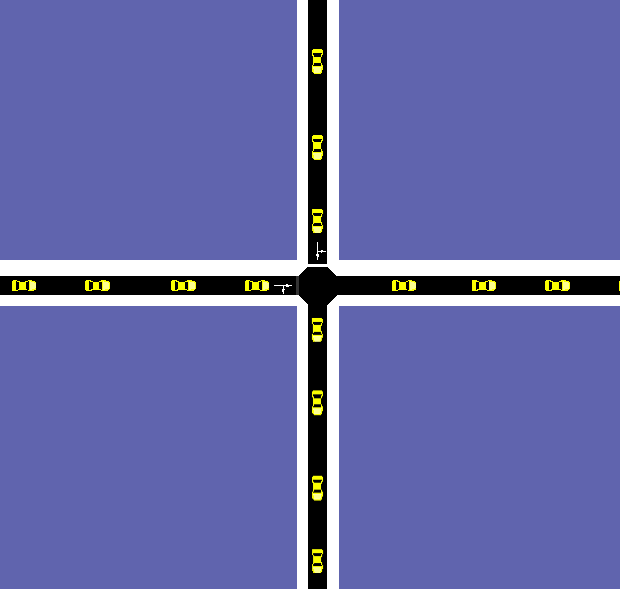
\includegraphics[width=.4\textwidth]{griglia-dettaglio-2.png}
% 	\end{center}
% 	\label{fig:griglia-dettaglio}\caption{Dettaglio della configurazione a griglia: in nero le strade e in giallo gli edifici.}
% \end{figure}
%
\subsection{Risultati}\label{sec:configurazione-griglia-risultati}
I grafici in \figurename~\ref{fig:risultati-griglia-copertura} mostrano il cambiamento della copertura dei veicoli in totale e sulla circonferenza,
dove si hanno rispettivamente $8064$ e $36$ veicoli, quando si vanno a considerare gli edifici.
Nelle simulazioni rappresentato a sinistra
Si può notare un generale calo della copertura causato dalla perdita di segnale per effetto dell'ombreggiatura,
anche se non significativo; la differenza è leggermente maggiore considerando solo i veicoli sulla circonferenza.
Analizzando invece il numero dei salti (\figurename~\ref{fig:risultati-griglia-salti}) necessari a raggiungere il perimetro della griglia
si nota un aumento generale di questo valore, leggermente maggiore con raggio trasmissivo $300$ metri.
Questo comporta che, mediamente, ci vogliono $1,104$ salti in più per raggiungere il perimetro se il raggio
trasmissivo è di $300$m, mentre ce ne vogliono $0,571$ se è di $500$m.
Il grafico in \figurename~\ref{fig:risultati-griglia-messaggi}) mostra un aumento del numero di messaggi
di inoltro inviati, in media, del $17,9$\% nel caso del raggio trasmissivo di $300$m
e del $163,9$\% nel secondo caso.
Combinando questi risultati con i precenti, si denota che, nel caso degli edifici,
un alto numero di pacchetti venga perso a causa della troppa attenuazione del segnale;
infatti per coprire (circa) la stessa percentuale di veicoli è necessario un numero molto maggiore di inoltri.
%
\begin{figure}[htbp]
	\centering
		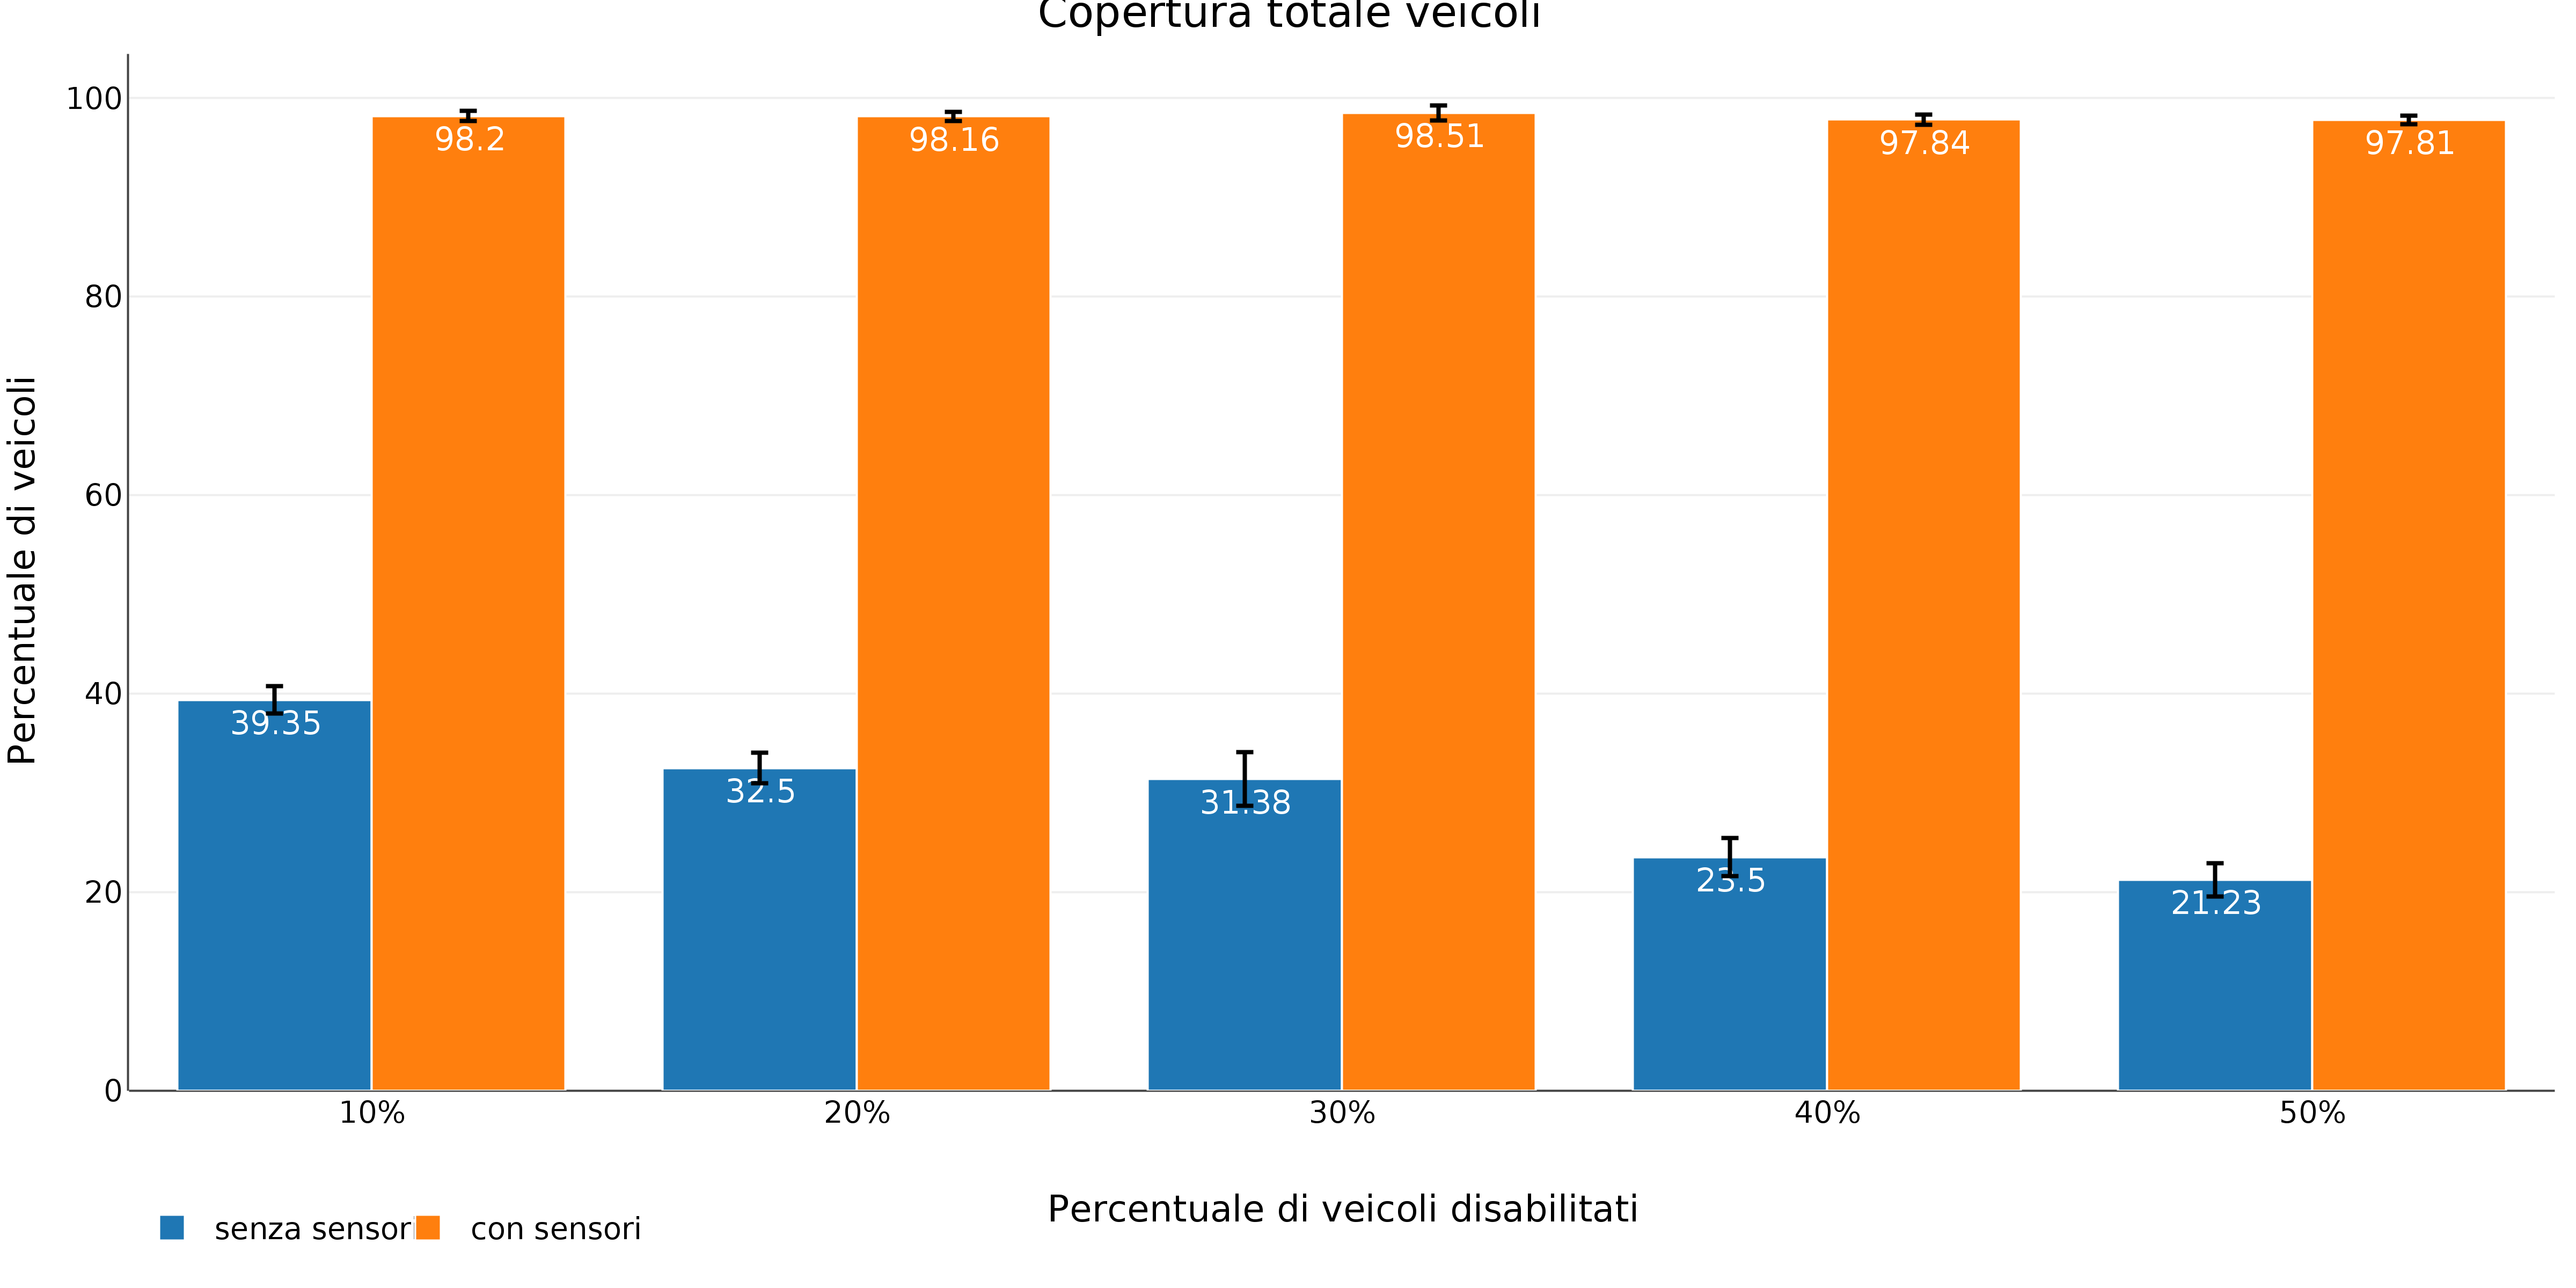
\includegraphics[width=\linewidth]{grafici/griglia/copertura_totale.png}
		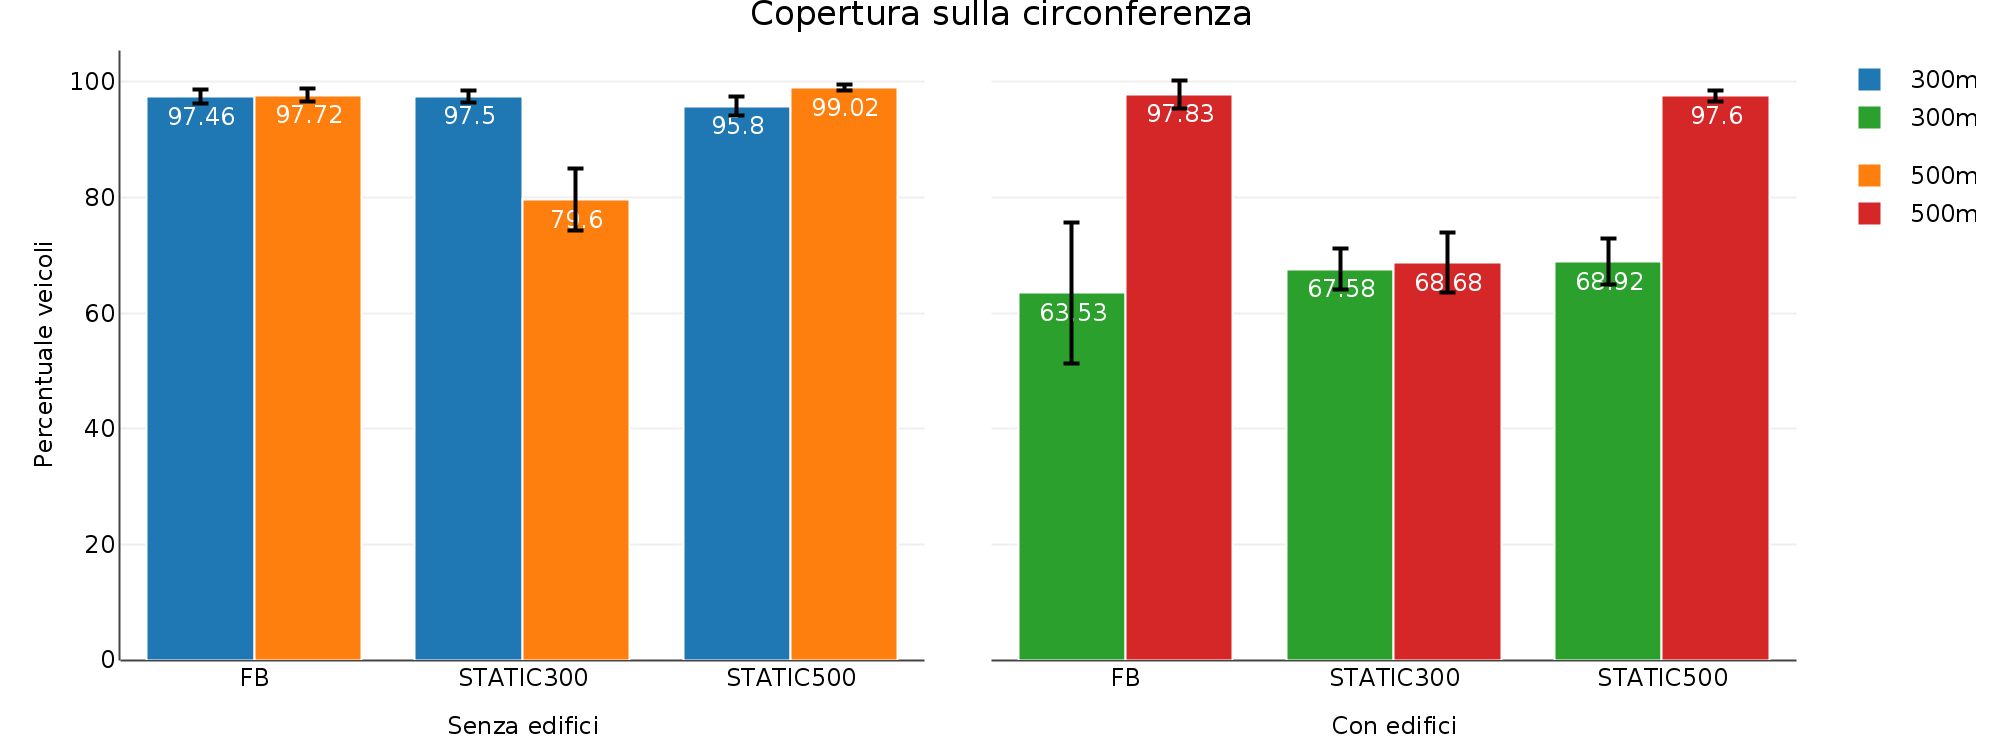
\includegraphics[width=\linewidth]{grafici/griglia/copertura_circonferenza.png}
\caption{Scenario a griglia: copertura dei veicoli totale e sulla circonferenza.\label{fig:risultati-griglia-copertura}}
\end{figure}
%
\begin{figure}[htbp]
	\centering
		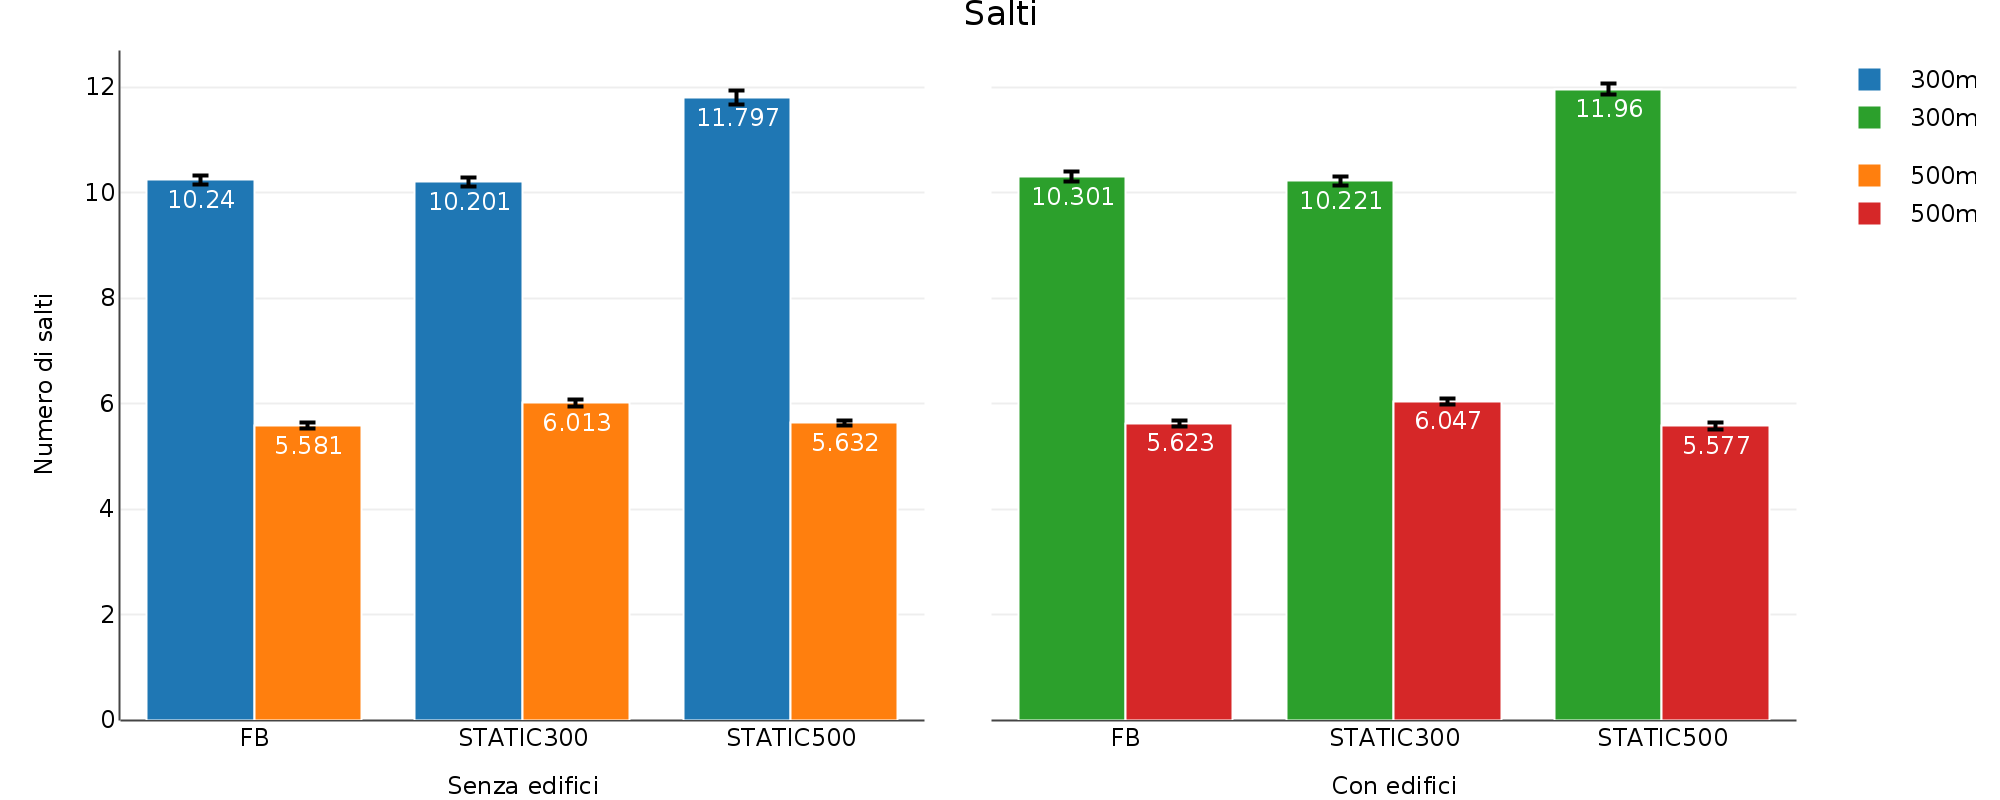
\includegraphics[width=\linewidth]{grafici/griglia/salti.png}
\caption{Scenario a griglia: numero di salti.\label{fig:risultati-griglia-salti}}
\end{figure}
%
\begin{figure}[htbp]
	\centering
		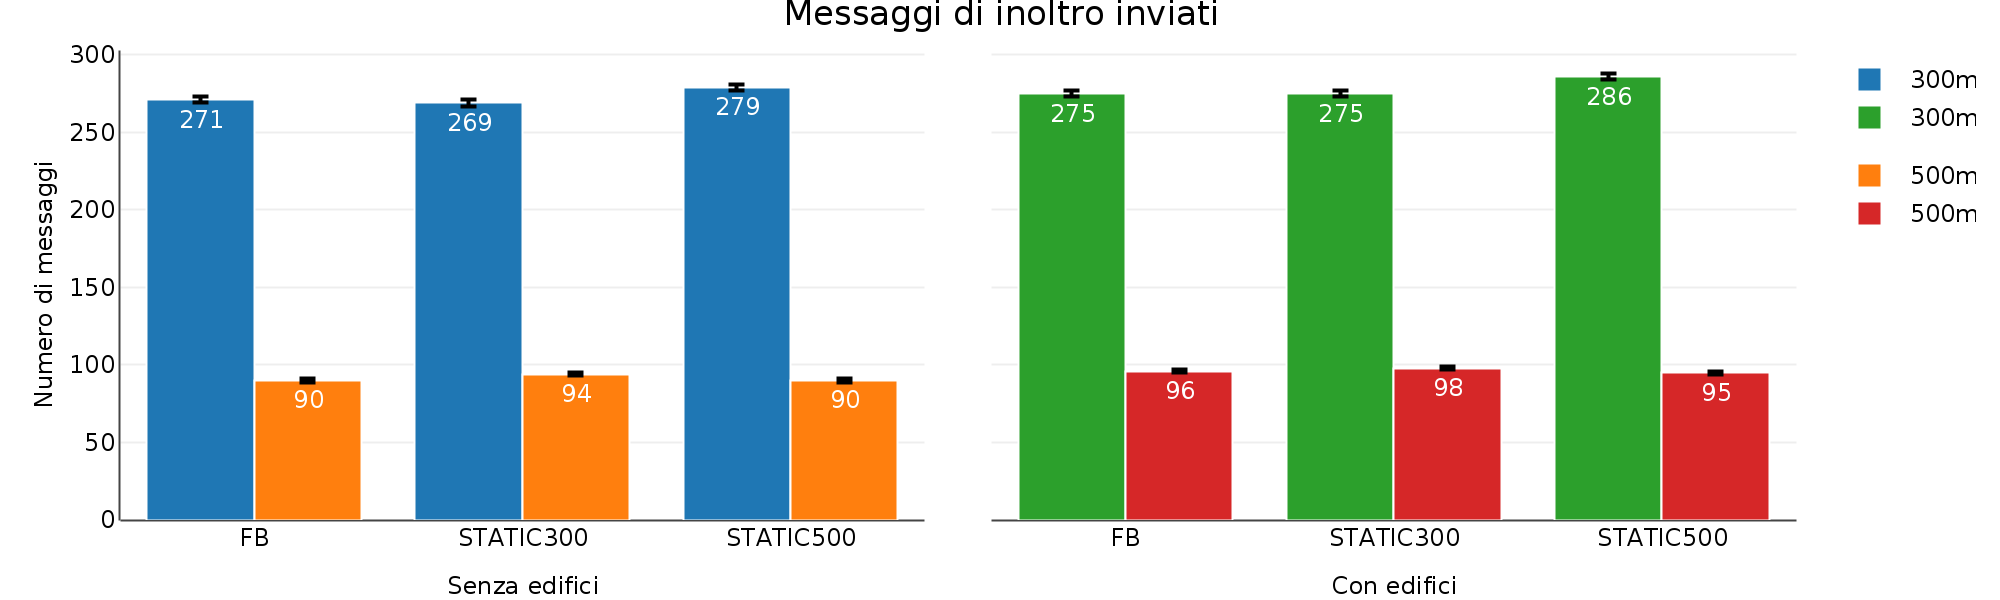
\includegraphics[width=\linewidth]{grafici/griglia/messaggi_inviati.png}
		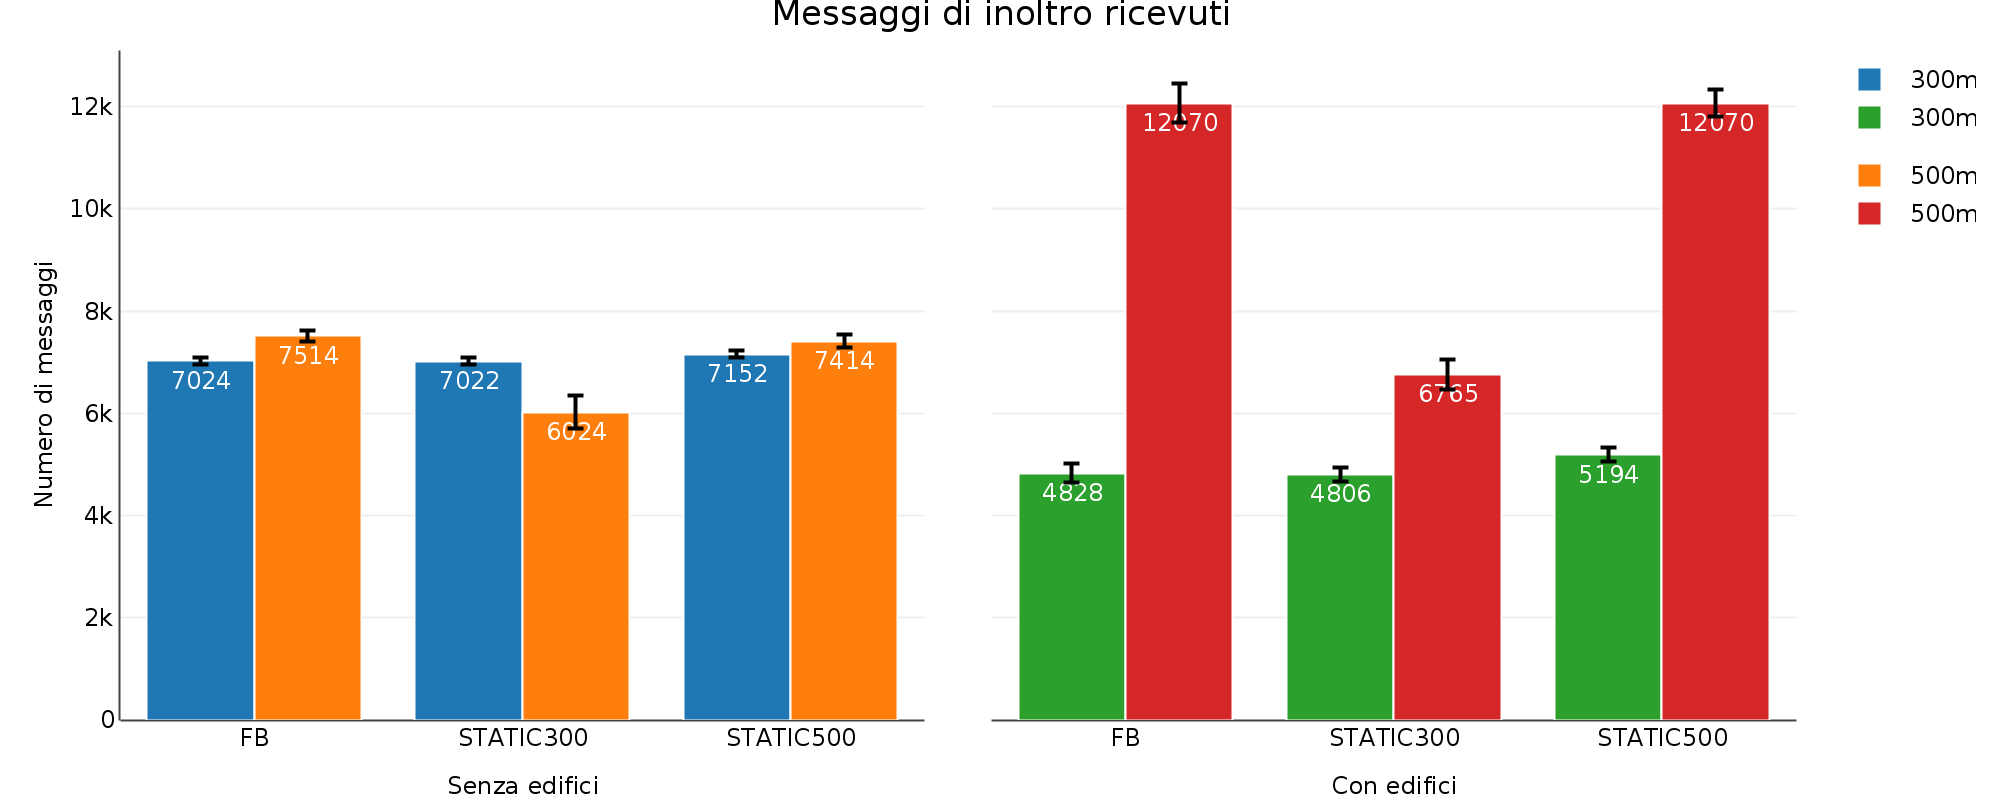
\includegraphics[width=\linewidth]{grafici/griglia/messaggi_ricevuti.png}
\caption{Scenario a griglia: numero di messaggi di inoltro inviati e ricevuti.\label{fig:risultati-griglia-messaggi}}
\end{figure}
%
%
\section{Scenario urbano reale} % un titolo migliore no?
Le configurazioni precedenti avevano il difetto di essere poco veritiere, sia dal punto di vista della topologia stradale
che sulla geometria degli edifici.
In questo gruppo di simulazioni, invece, si è voluto valutare Fast Broadcast all'interno di uno scenario quanto più reale possibile.
Sono state scelte due città, Padova (IT) e Los Angeles (California, USA) (Figura~\ref{fig:scenari-la-pd-osm}), definite due aree nella zona centrale di circa $5$ kilometri quadrati (Figura~\ref{fig:scenari-la-pd-osm})
e, seguendo il procedimento descritto nella Sezione~\ref{sec:sumo}, si sono estratte le informazioni necessarie alla simulazione.
Altre informazioni sulla configurazione sono elencati in Tabella~\ref{tab:parametri-simulazioni-pd-la}.

La scelta è ricaduta su Los Angeles poiché la sua rete stradale è molto simile a una griglia in stile Manhattan, come anche nello scenario precedente,
mentre Padova (sede anche dell'Università dove si è svolto questo lavoro) ha una toplogià più irregolare, con strade più strette ed edifici a ridosso di queste,
zone pedonali e ZTL.
%
\begin{table}[htbp]
	\centering
	  \begin{tabular}{| L{.35\linewidth} | C{.01\linewidth} | C{.04\linewidth} | L{.15\linewidth} | L{.15\linewidth} |}
			\toprule
			\multicolumn{3}{|m{.3\linewidth}|}{\multirow{2}{*}{}}														&		\multicolumn{2}{c|}{Scenario}						\\ \cline{4-5}
			\multicolumn{3}{|m{.3\linewidth}|}{}																						&		Padova				&			Los Angeles					\\
			\thickerline
			\multicolumn{2}{|m{.25\linewidth}|}{\multirow{2}{*}{Latitudine}}				&		N	 	& 	$45,4171$				&			$33,9654$					\\ \cline{3-5}
			\multicolumn{2}{|m{.25\linewidth}|}{}																		&		S	 	& 	$45,3981$				&			$33,9478$					\\ \hline
			\multicolumn{2}{|l|}{\multirow{2}{*}{Longitudine}}											&		O	 	& 	$11,8654$				&			-$118,3260$				\\ \cline{3-5}
			\multicolumn{2}{|l|}{}																									&		E	 	& 	$11,8923$				&			-$118,3055$				\\ \hline
			\multicolumn{3}{|l|}{Area approssimativa [km$^2$]}															&		\multicolumn{2}{c|}{$5$}								\\ \hline
			\multicolumn{3}{|l|}{Distanza fra veicoli [metri]}															&		\multicolumn{2}{c|}{$25$}								\\ \hline
			\multicolumn{3}{|l|}{Numero di veicoli}																					&		$2224$					&					$1905$				\\ \hline
			\multicolumn{3}{|l|}{Numero di edifici}																					&		$6322$					&					$8241$				\\ \hline
			\multicolumn{3}{|l|}{Circonferenza [metri]}																			&		\multicolumn{2}{c|}{$1000\pm25$}				\\ \hline
			\multicolumn{3}{|l|}{Posizione del veicolo zero}																&		\multicolumn{2}{c|}{centrale}						\\ \hline
			\multicolumn{3}{|l|}{Numero di simulazioni}																			&		\multicolumn{2}{c|}{$50$}								\\
			\bottomrule
	  \end{tabular}
	\caption{Parametri della topologia per gli scenari urbani.\label{tab:parametri-simulazioni-pd-la}}
\end{table}
%
\begin{figure}[htbp]
	\centering
		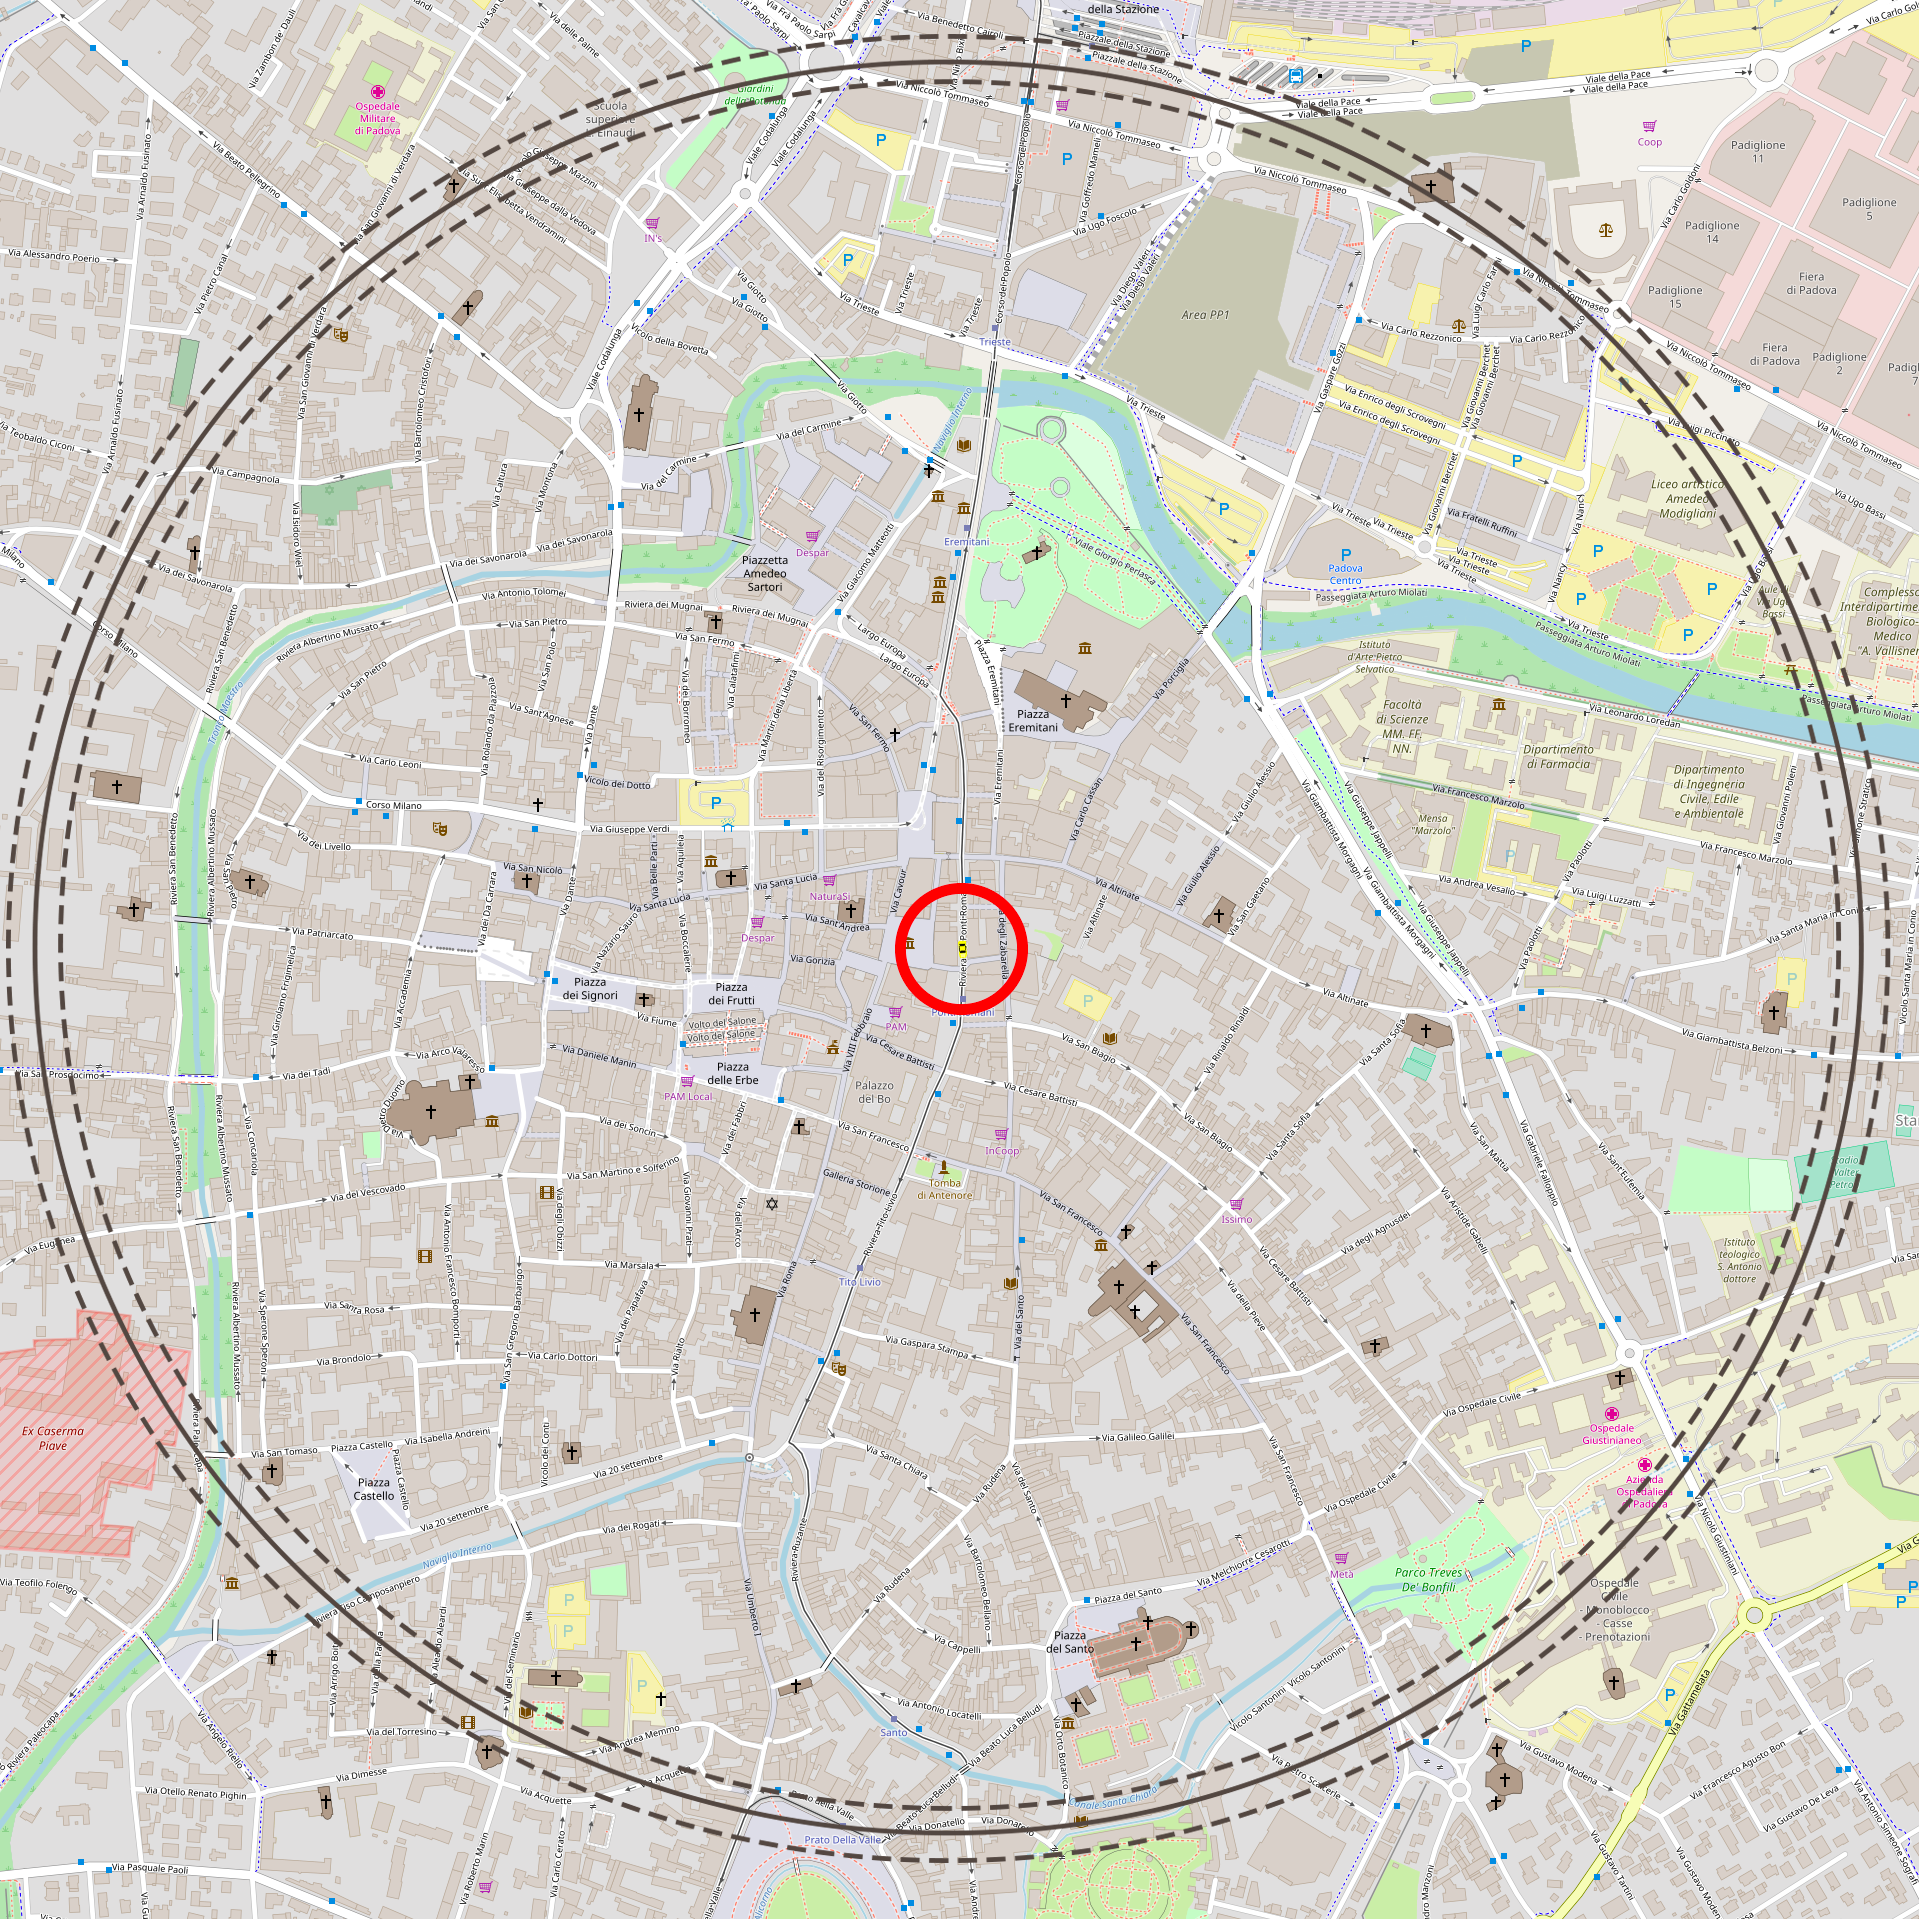
\includegraphics[width=.49\textwidth]{osm_web-pd-2x2.png}
		\hfill
		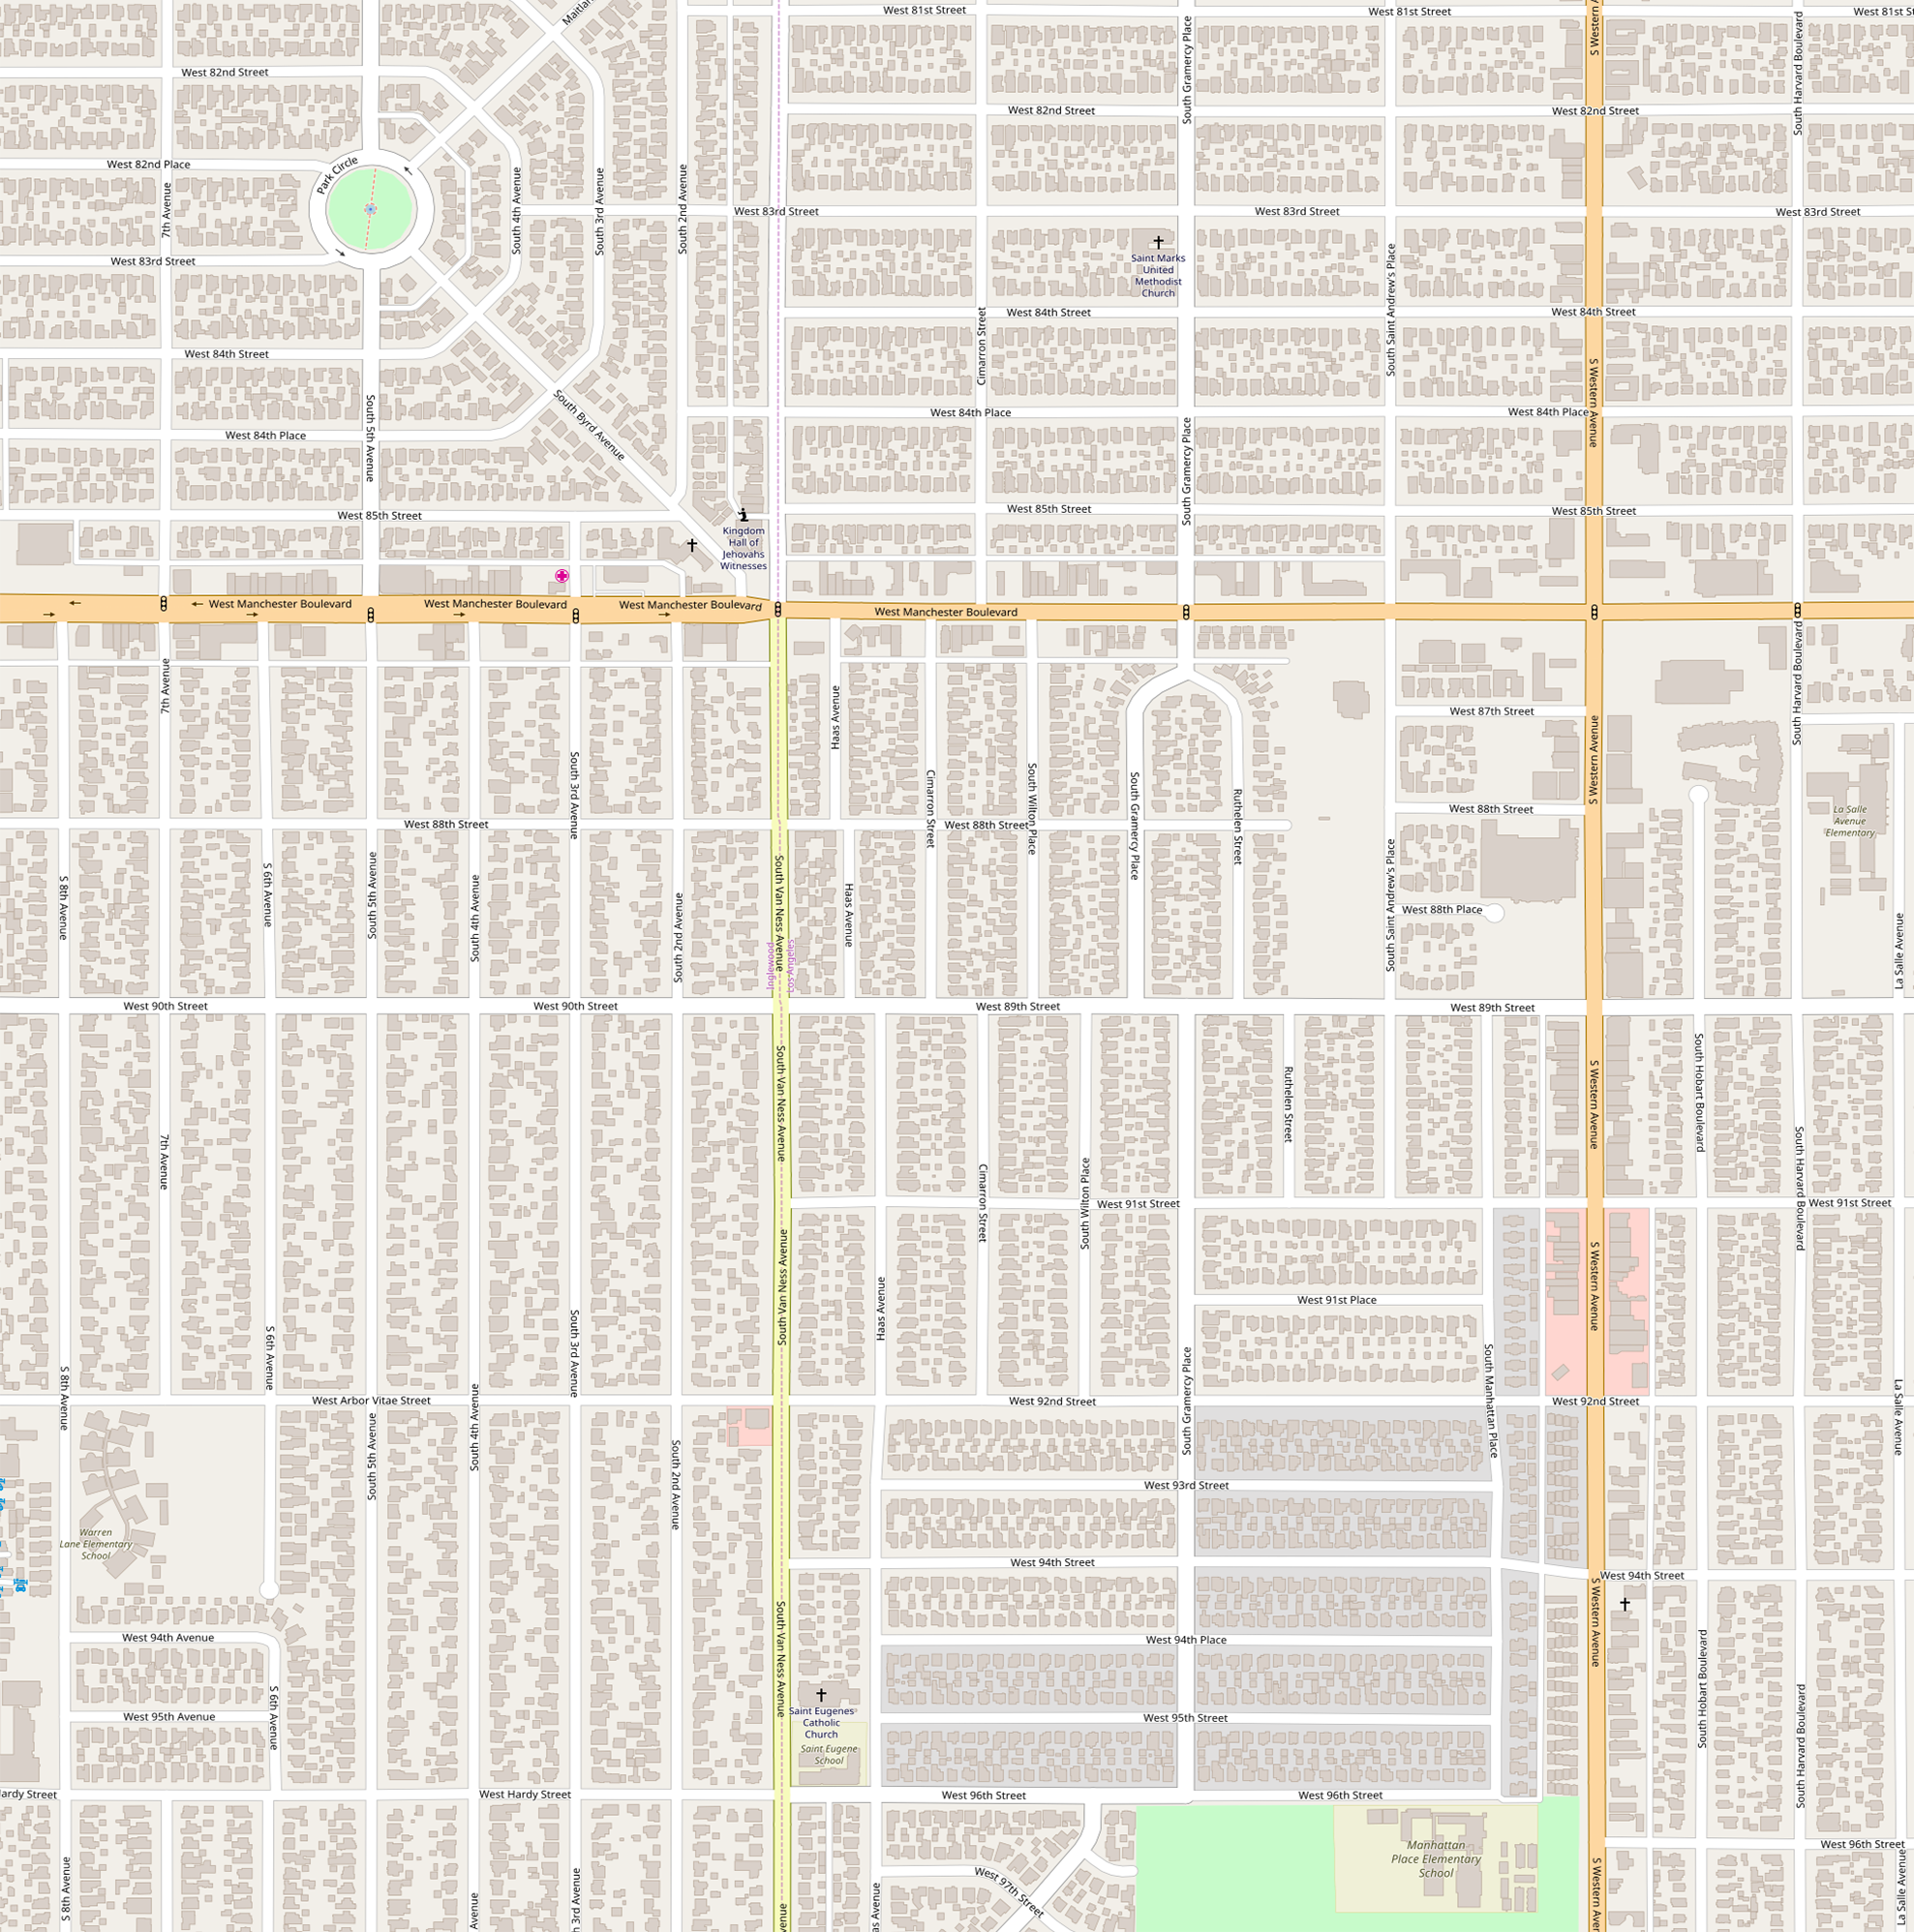
\includegraphics[width=.49\textwidth]{osm_web-la-2x2.png}
\caption{Una vista delle aree selezionate per le simulazioni; a sinistra la città di Padova e a destra Los Angeles (fonte: OSM).
Il cerchio rosso evidenzia la posizione del nodo di partenza mentre i tre rimanenti rappresentano il perimetro della circonferenza
e i due intervalli di confidenza.\label{fig:scenari-la-pd-osm}}
\end{figure}
%
Anche in questo gruppo di simulazioni sono state utilizzate le medesime metriche del caso precendente,
fatta eccezione per il numero di salti che ora sono per raggiungere la circonferenza, non il bordo dello scenario.
Questo perché nella configurazione a griglia lungo il perimetro esterno erano sicuramente posizionati dei veicoli,
mentre ora il limite ``quadratico'' dell'area è ideale (non tutte le strade finisco esattamente sul bordo della mappa).
%
\subsection{Los Angeles}\label{subsec:risultati-la}
%
\subsection{Padova}\label{subsec:risultati-pd}

% \begin{figure}[htbp]
% 	\centering
% 		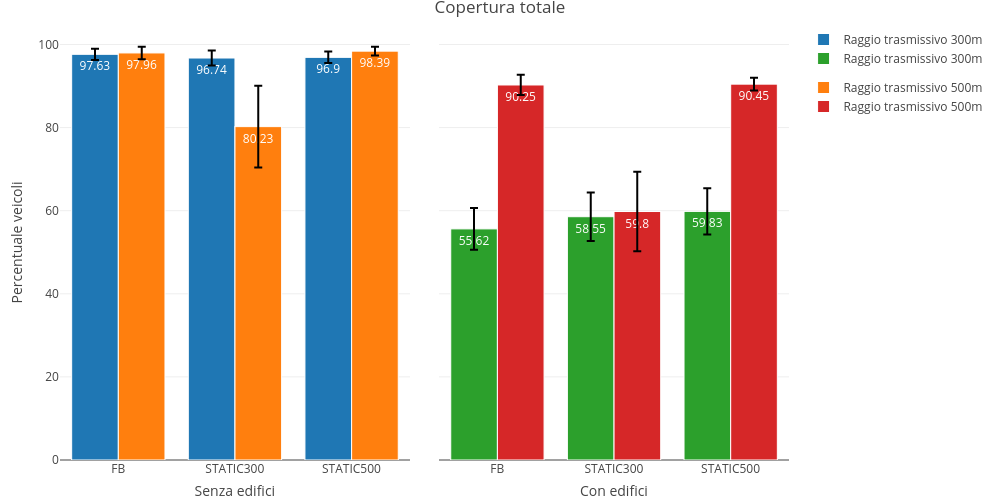
\includegraphics[width=\textwidth]{grafici/pd_copertura_totale.png}
% 		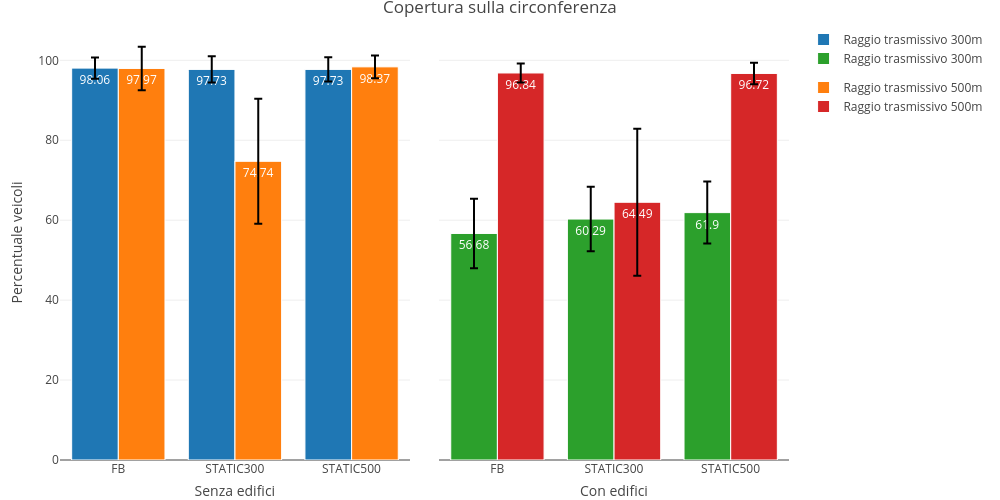
\includegraphics[width=\textwidth]{grafici/pd_copertura_circonferenza.png}
% \caption{Copertura dei veicoli totale e sulla circonferenza dei veicoli\label{fig:risultati-padova-copertura}}
% \end{figure}
% %
% \begin{figure}[htbp]
% 	\centering
% 		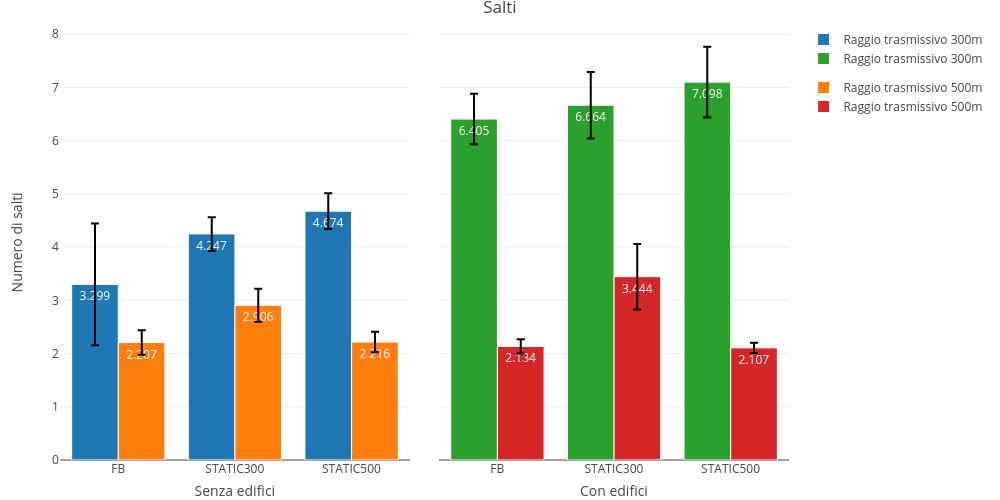
\includegraphics[width=\textwidth]{grafici/pd_salti.png}
% \caption{Numero di salti necessario per raggiungere la circonferenza dei veicoli\label{fig:risultati-padova-salti}}
% \end{figure}
% %
% \begin{figure}[htbp]
% 	\centering
% 		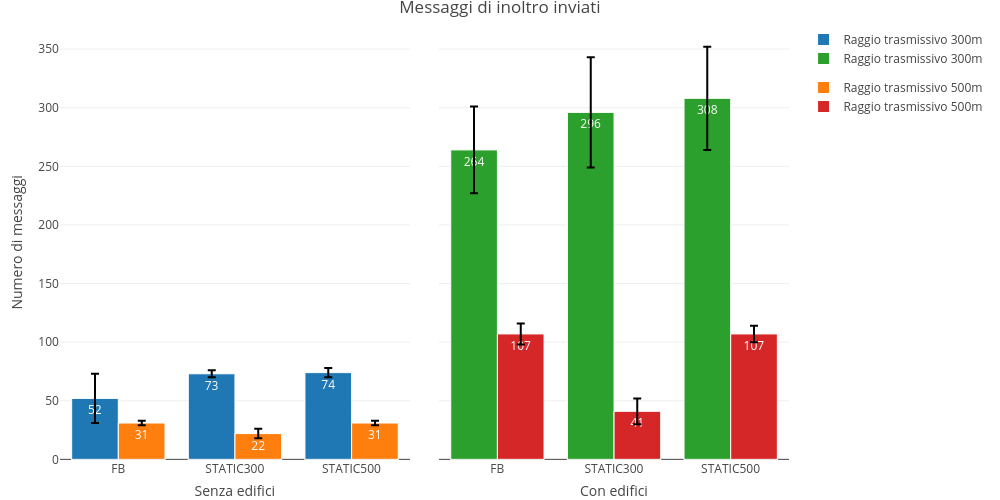
\includegraphics[width=\textwidth]{grafici/pd_messaggi_inviati.png}
% 		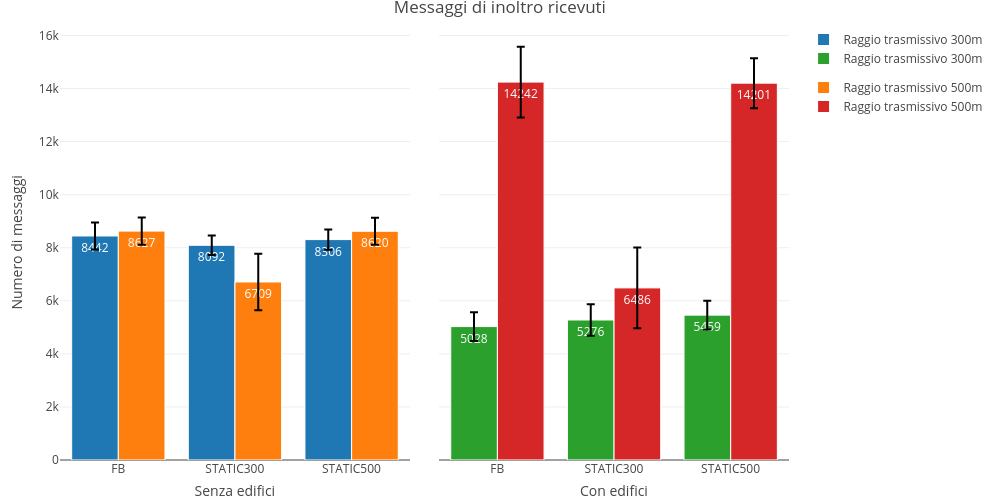
\includegraphics[width=\textwidth]{grafici/pd_messaggi_ricevuti.png}
% \caption{Quantità di messaggi di inoltro durante la simulazione.\label{fig:risultati-padova-messaggi}}
% \end{figure}


% BIBLIOGRAFIA
% \clearpage % da cambiare se prima ci sono troppi spazi vuoti
\bibliography{../utils/biblio.bib}
\bibliographystyle{ieeetr}

\end{document}
